\documentclass[12pt]{exam}
\usepackage[utf8]{inputenc}

\usepackage[margin=1in]{geometry}
\usepackage{amsmath,amssymb}
\usepackage{multicol}
\usepackage{mathrsfs}
\usepackage{graphicx}
\usepackage{multicol}
\usepackage[shortlabels]{enumitem}
\usepackage{scrextend}
\usepackage{xcolor}
\usepackage[normalem]{ulem}
\usepackage{optprog}

\newcommand{\class}{SA405, Fall 2021}
\newcommand{\term}{}
\newcommand{\examnum}{Final Exam}
\newcommand{\examdate}{14 December 2021}
\newcommand{\timelimit}{180 Minutes}

\pagestyle{head}
\firstpageheader{}{}{}
\runningheader{\class}{\examnum\ - Page \thepage\ of \numpages}{\examdate}
\runningheadrule

%% Answer box macros
%%\answerbox{alignment}{width}{height}
\newcommand{\answerbox}[3]{%
  \fbox{%
    \begin{minipage}[#1]{#2}
      \hfill\vspace{#3}
    \end{minipage}
  }
}

%%\answerboxfull{alignment}{height}
\newcommand{\answerboxfull}[2]{%
  \answerbox{#1}{6.38in}{#2} 
}

%%\answerboxone{alignment}{height} -- for first-level bullet
\newcommand{\answerboxone}[2]{%
  \answerbox{#1}{6.0in}{#2} 
}

%% special boxes
\newcommand{\wordbox}{\answerbox{c}{1.2in}{.7cm}}
\newcommand{\catbox}{\answerbox{c}{.5in}{.7cm}}
\newcommand{\letterbox}{\answerbox{c}{.7cm}{.7cm}}

\printanswers
%\noprintanswers
\begin{document}

\noindent
\begin{tabular*}{\textwidth}{l @{\extracolsep{\fill}} r @{\extracolsep{6pt}} r}
\textbf{\class} &&\textbf{\examnum}\\
\textbf{\term} &&\textbf{\examdate}\\
 && \\
 && \\
& \textbf{Name:} & \makebox[2.2in]{\hrulefill}\\\\
%\textbf{Time Limit: \timelimit} &  & \makebox[2in]{\hrulefill}
\end{tabular*}

\noindent
\rule[2ex]{\textwidth}{2pt}

%This exam contains \numpages\ pages (including this cover page) and \numquestions\ questions.\\
%Total of points is \numpoints.

\begin{itemize}
%\item You may pull the pages apart and then staple them together at the end.  I prefer not to see your name when I am grading, so only write your name on the first page (unless submitting pages unstapled).

\item %No books, notes, or any other outside help % or calculators
% that do symbolic manipulation (such as TI-89 or TI-92) 
 %allowed. %
 {\bf Two sided} 8.5 by 11 inch formula/note sheet is allowed.

%\item You may use your calculator on this test.

\item Show work clearly and neatly.  

\item Define all notation used.
%\item If you need more space than is provided, use the back of the previous page. 

\item Please read each question carefully.
If you are not sure what a question is
asking, ask for clarification.

\item If you start over on a problem, please CLEARLY indicate what your final
  answer is, along with its accompanying work.

%\item All formulations must have descriptions of any indices, parameters, and decision variables used. All constraints must be described. 
\end{itemize}

\bigskip
\begin{center}
Grade Table (for teacher use only)\\
\addpoints
\gradetable[v][questions]
\end{center}

\noindent
\rule[2ex]{\textwidth}{2pt}

% I think this is a requirement now
\emph{Please write the following statement and sign it.}\\
The Naval Service I am a part of is bound by honor
and integrity. I will not compromise our values by
giving or receiving unauthorized help on this exam.

\newpage %%%%%%%

% Adjust points as you'd like, we can make it add up to 100 when the whole thing is done

% Questions/Ideas/Topics: Not exhaustive
% \begin{itemize}
%     \item Langrangian Relaxation    \textit{\textbf{(Present in max form)}}
%     \item Branch and Bound \textit{\textbf{(Present)}}
%     \item Network Flow modeling
%     \begin{itemize}
%         \item Shortest path\textit{\textbf{(Present)}}
        
%         \item Maximum Flow\textit{\textbf{(Present)}}
%         \item Fixed-charge\textit{\textbf{(Present--kinda)}}
%         \item minimum cost flow \textit{\textbf{(Present--kinda)}}
%     \end{itemize}
%     \item Combinatorial model: TSP/VRP/MST \textit{\textbf{(Present)}} 
%     \item Facility location  \textit{\textbf{(Present--kinda)}}
%     \item Logical constraints maybe incorporate into others \textit{\textbf{( A few are Present)}}
%     \item IP formulations: maybe an easy multiple choice or something on convex hull/convex set/is a constraint valid \textit{\textbf{Present}}
% \end{itemize}

\newpage
% \textbf{Chris: I know this is shortest path, but I wonder what we will get if the mids do not identify it correctly}


\begin{questions}

% \question Suppose it costs \$10,000 to purchase a new car. The annual operating cost and resale value of a used care are shown in the table below. 

% \begin{center}
% \begin{tabular}{ccc} 
% Age (years) & Resale Value (\$) & Operating Cost (\$)\\\hline
% 1 & 7000 & 300 \\
% 2 & 6000 & 500\\
% 3 & 4000 & 800\\
% 4 & 3000 & 1200\\
% 5 & 2000 & 1600\\
% 6 & 1000 & 2200
% \end{tabular}
% \end{center}

% Assuming that one now has a new car, formulate an \textbf{\emph{abbreviated}} \textbf{\textit{concrete}} integer program for determining a replacement policy that minimizes the net cost of owning and operating a car for the next six years.
% \vfill

% \newpage

%  \textbf{Question: Is it required that each event is done? I was confused for the events if I should do >= 1 or ==2 since the mids are == 2}
\question The USNA Swim Team wants to match six of their swimmers to six events. The goal for the coach is to match swimmers with events in a way that maximizes the total compatibility of the six events. A value of 10 means that the swimmer is the most compatible with an event, and a value of 1 means that they are least compatible for an event. Each midshipman can swim up to two events, and each event must include at least one midshipman. The table below describes the compatibility of each swimmer with each event. 

\begin{center}
\begin{tabular}{c|ccccccc} 
Swimmer Name & 50m back & 100m back & 50m free & 100m free & 50m fly & 100m fly &  \\\hline
Micah & 2 & 3 & 4 & 4 & 8 & 9  \\
Ashley & 4 & 5 & 8 & 8 & 3 & 3 \\
Jamie & 9 & 8 & 3 & 2 & 1 & 1\\
Erin & 7 & 9& 5 & 4& 5 & 6\\
Katie & 8 & 10& 5 & 5& 3 & 3\\
Tim & 1 & 2& 5 & 3& 9 & 10
\end{tabular}
\end{center}

\begin{parts}

\part[3] Draw a network that makes it possible to represent the problem of maximizing the total compatibility of swimmer-event pairings. You don't necessarily need to draw and label \textit{all} arcs, for the sake of time.
\newpage
\part[7] Formulate the \emph{\textbf{parameterized}} integer program for solving the swim team coach's problem. Clearly define all sets, parameters, and variables.
\vfill
\end{parts}
\newpage

\question Each year, Dunder Mifflin produces as many as 400 printers in Albany and 300 printers in Utica. New York City customers must receive 400 printers and Buffalo customers must receive 300 printers. Producing a printer costs \$800 in Albany and \$900 in Utica. Computers are transported by plane may (but are not required to) be sent through Scranton. The costs of sending a printer between pairs of cities is shown in the table below.

\begin{center}
\begin{tabular}{cccc} 
From & To Scranton & To New York City & To Buffalo  \\\hline
Albany & \$80  & \$220 & \$280 \\
Utica & \$100  & \$140 & \$170\\
Scranton & - & \$40 & \$50
\end{tabular}
\end{center}

\begin{parts}
\part[6] Formulate an abbreviated concrete integer program that can be used to minimize the total cost of meeting Dunder Mifflin's annual demand. Clearly define all decision variables.
\newpage

\part[2] How would you modify the previous formulation if at most 200 units could be shipped through Scranton?

\vspace{2in}

Dunder Mifflin is interested in opening a new facility in Rochester. The cost to open this facility is a fixed cost of \$8000, and it costs \$50 to send a printer to Rochester from Albany or Utica, and it costs \$60 to send a printer from Rochester to New York City or Buffalo. Finally, if opened, Dunder Mifflin would be able to send at most 450 printers through Rochester.  How would you modify the previous formulation to consider this new decision? 

\part[2] What variables would you need to add?
\vspace{1in}
\part[2] How would you change the objective function?
\vfill
\part[3] What constraints should you add?
\vfill
\end{parts}
\newpage

% \textbf{Question: Do you want them to give subtour elim on this one? If so I would indicate it here like we did on Exam 2}
\question Michael Scott has decided to open up a new tech company, and he has five minicomputers across the city of Scranton. The distance between each pair of computers (in miles) is given in the following table. 

Assuming that the computers must be interconnected by underground cable, what is the minimum length of cable required? Note that if no distance between computers exists in the table, then cable cannot be connected between these two computers. 

\begin{center}
\begin{tabular}{cccccc} 
Computer & 1 & 2 & 3 & 4 & 5  \\\hline
1 & - & 1 & 4 & 6 & 2 \\
2 & 1 &  - & 2 &5 &5 \\
3 & 4 & 2  & - & 5 & 2 \\
4 & 6 & 5 & 5 & - & 4 \\
5 & 2 & 5 & 2 & 4 & - 
\end{tabular}
\end{center}

\begin{parts}
\part[6] Formulate an abbreviated \textit{\textbf{concrete}} integer program that solves Michael Scott's problem.
\vfill
\part[3] Subtour-elimination constraints are required for solving this problem. How many of them will exist or be needed? Give an example of one such constraint.
\vspace{1.5in}
\newpage
\part[2] Michael realizes that computer 3 can only be direct connected to, at most, one other computer. Modify your IP in order to include this restriction.

\vfill
\part[2] He also realizes that if computer 1 is directly connected to computer 2, then it must also be directly connected to computer 4. Modify your IP in order to include this restriction.

\vfill
\part[2] He also realizes that the number of computers directly connected to computer 5 must be \textbf{strictly} less than the number of computers directly connected to computer 4. \textbf{Using inequalities only}, modify your IP in order to include this restriction.
\end{parts}

\vfill

% Chris: Would it be possible/easy to number the nodes? It would make grading way easier for problems d and e
% If it's a pain don't bother
\newpage

\question Consider the following knapsack problem:
\begin{align*}
    \textrm {max } & 16x + 22y + 12w + 8z \\
    \textrm{s.t. } & 5x + 7y + 4w + 3z \le 14 \\
    & x,y,w,z \in \{0,1\} 
\end{align*}

Professors Curry and Lourenco are part of the way through solving this problem using the Branch-And-Bound algorithm. The figure below depicts their current progress within the B\&B tree. 

    \begin{center}
        
    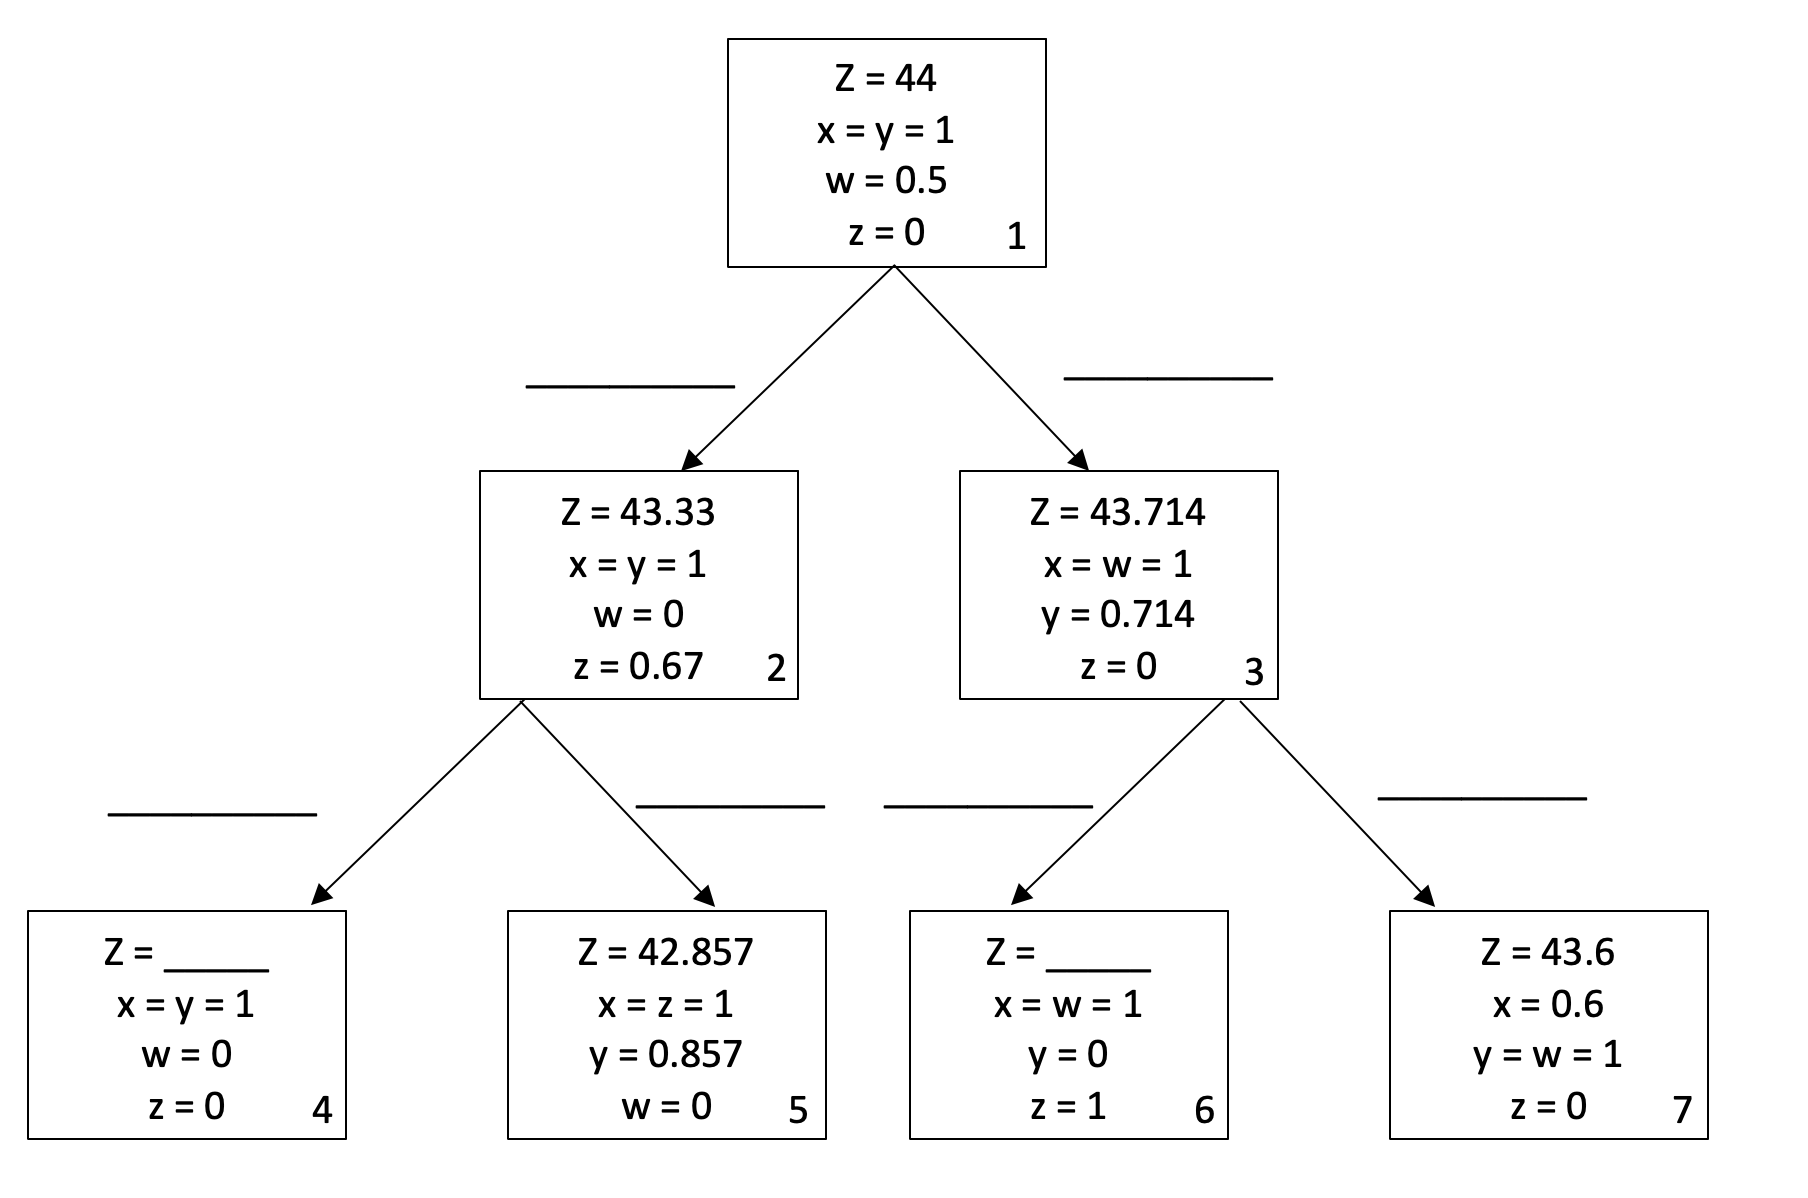
\includegraphics[width = .8\textwidth]{bandbfigure.png}
\end{center}
    
    
For this tree, answer the following questions:

\begin{parts}
\part[5] Fill in the blanks on the tree.
\vfill

\part[2] What's the current upper bound?
\vfill

\part[2] What's the current lower bound?
\vfill

\part[2] Which nodes are \emph{active}?
\vfill

\part[2] Which nodes have been or should be \emph{pruned}?

\vfill
\part[4] Should you continue branching? If so, draw the new branches on the tree.
\vfill
\end{parts}

\newpage
%\question Multiple Choice question: Lagrangian Relaxation \& IP Formulations--Chris?

% This is a convex sets picture but I removed it
%\part[2] Which of the following sets are Convex?
%\begin{center}
%    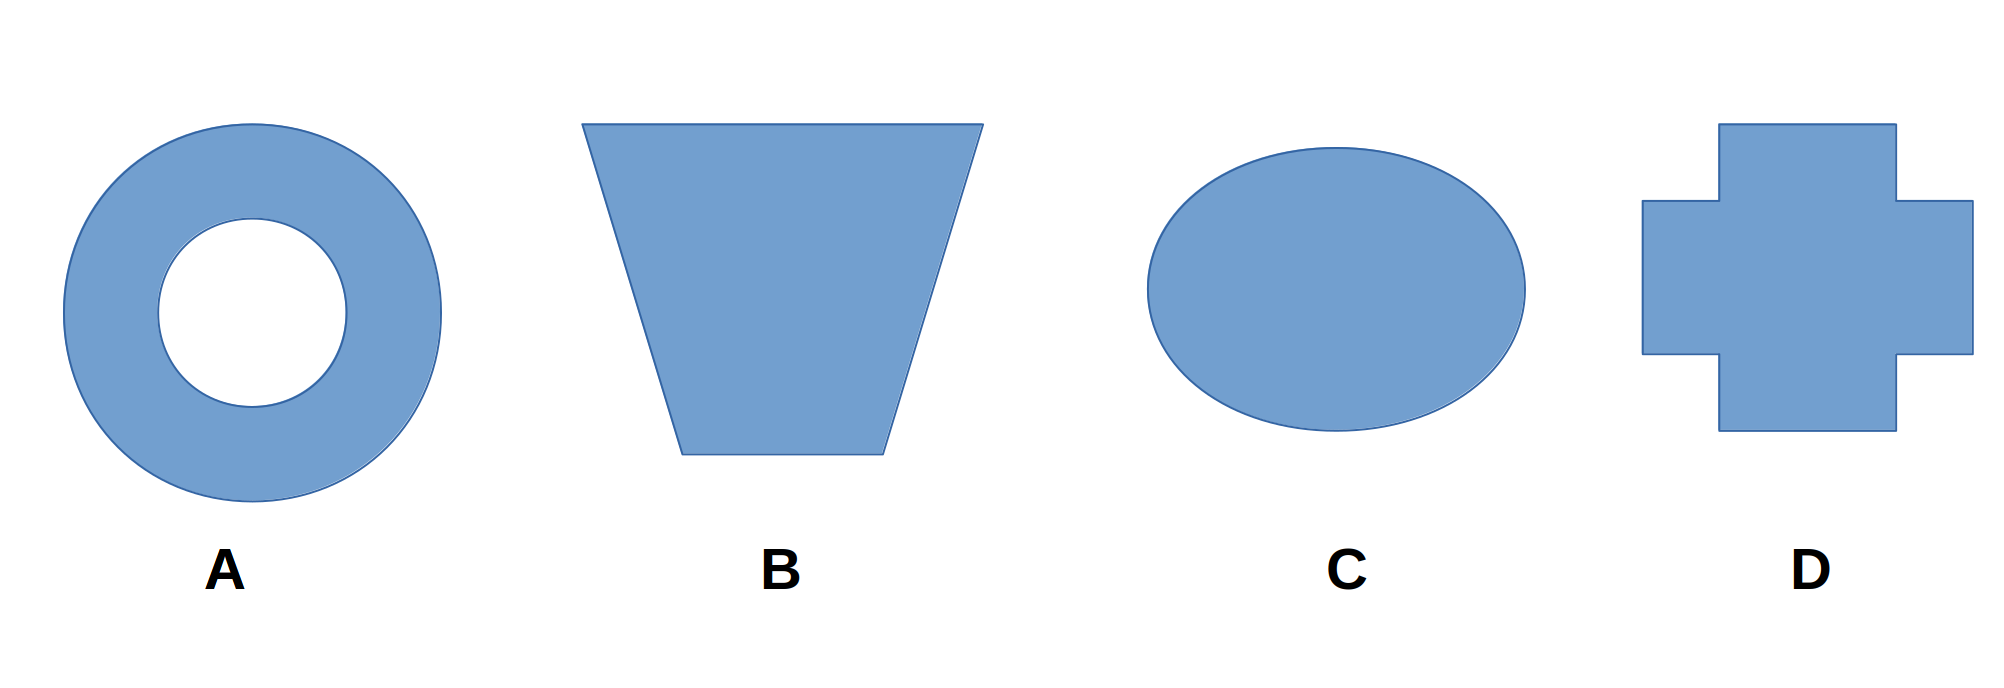
\includegraphics[width=4in]{ConvexSets.png}
%\end{center}

\question Consider the following Integer Program:
\begin{optprog}
max &\objective{ 2 x_1 + 3 x_2 - 4 x_3} \\ 
st & x_1 + x_2 + 2 x_3 & \leq & 7 \\
   & x_2 + x_3         & \geq  & 1 \\
   & x_1               & \leq & 5 \\
   & x_1               & \geq & 0 \text{, integer} \\
   & x_2, x_3          & \in & \{0,1\}
\end{optprog}
\begin{parts}
\part[2] Does the constraint $x_1 + x_2 + x_3 \leq 3$ violate the feasible region of the integer program above? Briefly explain why or why not. \vfill
\part[2] Does the constraint $x_2 + x_3 \leq 2$ violate the feasible region of the integer program above? Briefly explain why or why not \vfill
\part[2] Suppose I wanted to solve this problem with Lagrangian Relaxation. I want to relax constraint (2) from the feasible region (that is $x_1 + x_2 + 2 x_3 \leq 7$). What is the objective function of this Lagrangian Relaxation? \vfill
\part[2] I still want to apply Lagrangian Relaxation, but this time I want to relax constraint (3) (that is $x_2 + x_3 \geq 1$). What is the objective function of the Lagrangian Relaxation? \vfill
\part[2] Suppose I solve the LP relaxation of this integer program. The solution I obtain is $(x_1,x_2,x_3) = (5,1,0.5)$ with objective function value $z = 11$. What does this tell me about the objective function value of the original IP? \vfill
\part[1] Is the feasible region of this IP a convex set? \hfill YES \hspace{0.5cm} NO
\part[1] Is the feasible region of the LP relaxation a convex set?  \hfill YES \hspace{0.5cm} NO
\part[1] Are the feasible regions of the Lagrangian Relaxations defined above convex sets? \newline \phantom{a} \hfill YES \hspace{0.5cm} NO
\end{parts}
\newpage

\question The Navy is determining where to place some sensors to monitor information in an undersea network. The network below shows the 10 locations that must be covered.
\begin{center}
    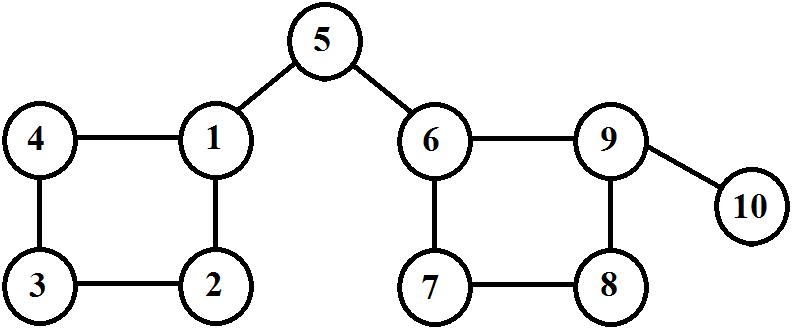
\includegraphics[width=0.6\textwidth]{10nodegraph.png}
\end{center}

A node is the network is covered if a sensor is installed in either its location or a node to which it's connected. Each sensor costs \$2000 to install. Lastly, each potential sensor location processes the following number of bits (regardless of where it comes from and based on the wiring in that area) given in the table below:

\begin{center}
\begin{tabular}{c|cccccccccc} 
Node & 1 & 2 & 3 & 4 & 5 & 6 & 7 & 8 & 9 & 10  \\\hline
Bits Processed & 175 & 235 & 220 & 180 & 205 & 190 & 200 & 215 & 195 & 215
\end{tabular}
\end{center}

The network must be able to process at least 700 bits of information across all sensors.

To get started, they have defined the following variables.

\textbf{\underline{Decision Variables}}

Let $x_n = 1$ if a sensor is placed at node $n$ for all $n \in \{1,2,3,\hdots,10\}$.

\begin{parts}
\part[8] Using the variables defined above, write a concrete model which ensures that each node in the network is covered while processing at least 700 bits of information among all installed sensors at minimum cost.

\newpage

\part[7] The Navy is considering upgrading their wiring infrastructure for the sensor network. To upgrade the wires, it would cost \$2500; however, it would increase the capability of each sensor to process 100 additional bits (thus, if they upgrade the wiring sensor 1 can process 275, sensor 2 can process 335, etc). How would the model change to incorporate this potential new decision? Make sure you clearly define any new variable(s) used and clearly show how this new change affects your objective function and/or the constraints.
\end{parts}

\newpage

\question Professor Lourenco is going to Busch Gardens Christmas Town to celebrate the end of the semester. There are eight major attractions he wants to see: Appolo's Chariot (A), Christmas Town Express (C), Elmo's Christmas (E), Invadr (I), Oktoberfest (O), Pictures with Santa (S), Verbolten (V), and Wine Tasting (W). The distances (in miles) between each of these 8 attractions are given in the table below:

\begin{center}
\begin{tabular}{ccccccccc} 
  & A & C   & E   & I   & O   & S   & V    & W  \\\hline
A & - & 1.1 & 1.4 & 1.6 & 0.7 & 0.4 & 1.3  & 1.1 \\
C & - & -   & 0.7 & 1.1 & 0.3 & 2.1 & 0.5 & 1.9 \\
E & - & -   & -   & 0.6 & 1.1 & 0.7 & 1.2 & 0.9 \\
I & - & -   & -   & -   & 1.0 & 1.2 & 0.8 & 0.6 \\
O & - & -   & -   & -   & -   & 1.1 & 0.9 & 1.1 \\
S & - & -   & -   & -   & -   & -   & 0.7 & 1.1 \\
V & - & -   & -   & -   & -   & -   & -   & 1.5 \\
W & - & -   & -   & -   & -   & -   & -   & - \\
\end{tabular}
\end{center}

\begin{parts}
\part[5] Since Elmo's Christmas is closest to the entrance, he decides to start there. Starting from Elmo's Christmas, formulate a concrete model which would allow Professor Lourenco to visit all of the 8 attractions and return to his starting point while walking as little as possible. If your model has an exponential number of constraints, do \textbf{not} include them here. 
\newpage
\part Suppose that you solved the problem above and you retrieved the following solution:

\verb|You should select edges (A,E), (A,V), (C,S), (C,W), (E,I), (I,V),|

\verb|(O,S), (O,W)|
    \begin{subparts}
    \subpart[2] What are the values of the variables associated with this solution? \vfill
    \subpart[1] Is this solution optimal to your problem? \vfill
    \subpart[3] If the solution is optimal, explain why. If the solution is not optimal, write which constraint(s), in concrete form, you would add to your model to remove this solution from the feasible region. \vfill
    \end{subparts}
\newpage
\part[4] Professor Lourenco realizes that he forgot to consider how picturesque the park is due to the light displays. He now assigns a ``picturesque factor'' for each of the walks between attractions given in the table below:
\begin{center}
\begin{tabular}{ccccccccc} 
  & A & C   & E   & I   & O   & S   & V    & W  \\\hline
A & - & 7   & 8   & 4   & 6   & 3   & 10   & 1 \\
C & - & -   & 7   & 2   & 4   & 1   & 5    & 9 \\
E & - & -   & -   & 6   & 3   & 4   & 5    & 2 \\
I & - & -   & -   & -   & 1   & 2   & 8    & 5 \\
O & - & -   & -   & -   & -   & 3   & 7    & 4 \\
S & - & -   & -   & -   & -   & -   & 4    & 1 \\
V & - & -   & -   & -   & -   & -   & -    & 5 \\
W & - & -   & -   & -   & -   & -   & -    & - \\
\end{tabular}
\end{center}

He now decides that he wants to visit all of the attractions while having as picturesque of a walk as possible. That said, he is willing to walk only a maximum of 10 miles to do so. How would your model from part (a) change to reflect this new goal?

\end{parts}


\end{questions}
\end{document}
